
%%%%%%%%%%%%%%%%%%%%%%%%%%%%%%%%%%%%%%%%%%%%%%%%%%%%%%%%%%%%%%%%%%%%%%%%%%%% 
% AGUJournalTemplate.tex: this template file is for articles formatted with LaTeX
% 
% This file includes commands and instructions
% given in the order necessary to produce a final output that will
% satisfy AGU requirements, including customized APA reference formatting.
% 
% You may copy this file and give it your
% article name, and enter your text.
% 
% 
% Step 1: Set the \documentclass
% 
% 

%% To submit your paper:
\documentclass[draft]{agujournal2019}
\usepackage{url} %this package should fix any errors with URLs in refs.
\usepackage{lineno}
\usepackage{hyphenat}
\usepackage{float}
\usepackage{multirow}
\usepackage[inline]{trackchanges} %for better track changes. finalnew option will compile document with changes incorporated.
\usepackage{soul}
\usepackage{array}
\newcolumntype{L}[1]{>{\raggedright\arraybackslash}p{#1}}
\newcolumntype{C}[1]{>{\centering\arraybackslash\hspace{0pt}}p{#1}}

\linenumbers
\sloppy
\hbadness=99999 
%%%%%%% 
% As of 2018 we recommend use of the TrackChanges package to mark revisions.
% The trackchanges package adds five new LaTeX commands:
% 
% \note[editor]{The note}
% \annote[editor]{Text to annotate}{The note}
% \add[editor]{Text to add}
% \remove[editor]{Text to remove}
% \change[editor]{Text to remove}{Text to add}
% 
% complete documentation is here: http://trackchanges.sourceforge.net/
%%%%%%% 

\draftfalse

%% Enter journal name below.
%% Choose from this list of Journals:
% 
% JGR: Atmospheres
% JGR: Biogeosciences
% JGR: Earth Surface
% JGR: Oceans
% JGR: Planets
% JGR: Solid Earth
% JGR: Space Physics
% Global Biogeochemical Cycles
% Geophysical Research Letters
% Paleoceanography and Paleoclimatology
% Radio Science
% Reviews of Geophysics
% Tectonics
% Space Weather
% Water Resources Research
% Geochemistry, Geophysics, Geosystems
% Journal of Advances in Modeling Earth Systems (JAMES)
% Earth's Future
% Earth and Space Science
% Geohealth
% 
% ie, \journalname{Water Resources Research}

\journalname{Geophysical Research Letters}

\newcommand{\aref}[1]{\textbf{Reference #1}}
\newcommand{\TODO}[1]{\textbf{TODO #1}}
\newcommand{\ian}[1]{{\textbf{\color{blue}Ian says:} \color{blue} #1} }
\newcommand{\leif}[1]{{\textbf{\color{red}Leif says:} \color{red} #1} }
\newcommand{\db}{\textit{DEBRIS}\,}
\newcommand{\cl}{\textit{CLEAN}\,}
\newcommand{\m}{$\,\mathrm{m}$\,}
\newcommand{\cm}{$\,\mathrm{cm}$\,}
\newcommand{\mma}{$\,\mathrm{mm  \, a^{-1}}$\,}
\newcommand{\mmma}{$\,\mathrm{m^3\, a^{-1}}$\,}
\newcommand{\mmms}{$\,\mathrm{m^3\, s^{-1}}$\,}
\newcommand{\unit}[1]{$\mathrm{#1}$}


\newenvironment{laysummary}{
  \chapter{\centering \textbf{Plain Language Summary}}
}



\begin{document}
%% ------------------------------------------------------------------------ %%
% Title
% 
% (A title should be specific, informative, and brief. Use
% abbreviations only if they are defined in the abstract. Titles that
% start with general keywords then specific terms are optimized in
% searches)
% 
%% ------------------------------------------------------------------------ %%

% Example: \title{This is a test title}


\title{Water discharge has a variable impact on sediment transport capacity in subglacial systems} 


\ian{Alpine glacier vs Ice sheet}

%% ------------------------------------------------------------------------ %%
% 
% AUTHORS AND AFFILIATIONS
% 

% Authors are individuals who have significantly contributed to the
% research and preparation of the article. Group authors are allowed, if
% each author in the group is separately identified in an appendix.)

% List authors by first name or initial followed by last name and
% separated by commas. Use \affil{} to number affiliations, and
% \thanks{} for author notes.
% Additional author notes should be indicated with \thanks{} (for
% example, for current addresses).

% Example: \authors{A. B. Author\affil{1}\thanks{Current address, Antarctica}, B. C. Author\affil{2,3}, and D. E.
% Author\affil{3,4}\thanks{Also funded by Monsanto.}}

\authors{Ian Delaney\affil{1}}


\affiliation{1}{Institut des dynamiques de la surface terrestre (IDYST), Universit\'{e} de Lausanne, B\^{a}timent G\'{e}opolis, CH-1015 Lausanne }

% \affiliation{3}{Third Affiliation}
% \affiliation{4}{Fourth Affiliation}

% \affiliation{=number=}{=Affiliation Address=}
% (repeat as many times as is necessary)

%% Corresponding Author:
% Corresponding author mailing address and e-mail address:

% (include name and email addresses of the corresponding author.  More
% than one corresponding author is allowed in this LaTeX file and for
% publication; but only one corresponding author is allowed in our
% editorial system.)

% Example: \correspondingauthor{First and Last Name}{email@address.edu}

\correspondingauthor{Ian Delaney}{ianarburua.delaney@unil.ch}



%% Keypoints, final entry on title page.

% List up to three key points (at least one is required)
% Key Points summarize the main points and conclusions of the article
% Each must be 140 characters or fewer with no special characters or punctuation and must be complete sentences

% Example:
% \begin{keypoints}
% \item	List up to three key points (at least one is required)
% \item	Key Points summarize the main points and conclusions of the article
% \item	Each must be 140 characters or fewer with no special characters or punctuation and must be complete sentences
% \end{keypoints}



\begin{keypoints}
\item Water discharge variations in subglacial channels are mainly accommodated by water velocity, not channel size, given their slow evolution.

\item Greater variability in water velocity in subglacial systems causes sediment transport capacity to vary more than subaerial systems.

\item The systems' divergence in transport response may impact sediment dynamics at glacier margins and interpretation of sediment records.
\end{keypoints}


%% ------------------------------------------------------------------------ %%
% 
% ABSTRACT and PLAIN LANGUAGE SUMMARY
% 
% A good Abstract will begin with a short description of the problem
% being addressed, briefly describe the new data or analyses, then
% briefly states the main conclusion(s) and how they are supported and\cite <e.g.,>[and others]{lewin76}
% uncertainties.

% The Plain Language Summary should be written for a broad audience,
% including journalists and the science-interested public, that will not have 
% a background in your field.
% 
% A Plain Language Summary is required in GRL, JGR: Planets, JGR: Biogeosciences,
% JGR: Oceans, G-Cubed, Reviews of Geophysics, and JAMES.
% see http://sharingscience.agu.org/creating-plain-language-summary/)
% 
%% ------------------------------------------------------------------------ %%

%% \begin{abstract} starts the second page 

\begin{abstract} % 150 words
  

In both subglacial and subaerial channels, sediment transport capacity of a sediment size depends mainly on 1) the channel width over which the sediment is mobilized  and 2) the shear stress applied by flowing water on sediment at the channel bottom; the shear stress depends mainly on the water velocity.
In subaerial channels, changing water discharge will  change the water depth,  the channel width (which dictates the distance  over which sediment transport  occurs), and the  water velocity (which controls the sediment transport capacity).
In subglacial environments, however, on times scales of hours to weeks, changing water discharge will only alter  water velocity, not channel area, because the subglacial conduit maintains a largely fixed geometry.
The fixed conduit geometry also means that the channel width over which the sediment is  mobilized also does not respond to changing water discharge.
Parameterizations of these processes show that sediment transport capacity varies far more in subglacial systems compared to subaerial systems, even though changing channel width can accommodate some sediment transport variability in subaerial channels.
The increased variability in sediment transport capacity in subglacial systems, compared to subaerial ones, has several important implications for sediment transport processes in glacierized catchments and the interpretation of sediment discharge records.

\end{abstract}

%% ------------------------------------------------------------------------ %%
% 
% TEXT
% 
%% ------------------------------------------------------------------------ %%

%%% Suggested section heads:
\ian{comparison with Alley 1997... mention his variability-- also deal with his $Qs \propto Qw^{\frac{9}{2}}$  treats like rivers?  does not consider channel size evolution}

\section{Introduction}
\label{sect:intro}


Glaciers expel large quantities of sediment from their termini \cite{hallet1996}.
Changes in glacier dynamics, geomorphology, and hydrology  have prompted numerous  recent studies of  sediment transport processes in cold regions \cite<e.g.>[]{zhang2022}.
Increases in sediment transport  have been observed in Greenland \cite{bendixen2017}, the European Alps \cite{costa2017}, the Himalayas \cite{li2021}, and the Andes \cite{vergara2022}.
In some of these regions, increased water discharge and glacier melt have been attributed to greater sediment transport capacity \cite{bendixen2017,costa2017,li2021}.
In other cases, enhanced access of meltwater to subglacial sediment at high elevations was attributed as the cause of increased sediment transport \cite{delaney2020,vergara2022}.
Observed changes to sediment transport in glacierized catchments create an imperative to examine the processes controlling sediment discharge here. 
Yet, the relationship between water discharge and sediment transport in subglacial environments remains minimally discussed and not contrasted with the subaerial river systems that these glaciers feed.

Over long periods, processes such as glacier abrasion and quarrying sculpt landscapes and create sediment to be transported fluvially from below glaciers \cite<c.f.>{hallet1979,iverson2012,ugelvig2018}. 
On shorter time periods, pressurized water transports sediment from the below glacier \cite{walder1994,creyts2013,beaud2018}, should enough sediment be present below the glacier (i.e. in a transport-limited regime).

In a transport-limited regime, sediment discharge responds to the sediment transport capacity or the amount of sediment that could be carried by the water. Sediment transport capacity depends on the shear stress between water and sediment it flows  over \cite{shields1936,meyer1948,engelund1967} and the width of the channel bottom $w_c$ over which to mobilize sediment. The shear stress  across the channel width $\tau_t$ responds to the velocity of water $v$ flowing through at channel so that 
\begin{linenomath*}
  \begin{equation}
    \label{eq:tau_t}
    \tau_t \propto w_c\, v^2,
  \end{equation}
\end{linenomath*}
% 
where $w_c$ is the width of the channel.
Following the conservation of mass, the velocity of the water flowing through a  channel is given as 
\begin{linenomath*}
  \begin{equation}
    \label{eq:v}
    v = \frac{Q_w}{S},
  \end{equation}
\end{linenomath*}
% 
where $Q_w$ is water discharge,  and $S$ is the channel's cross-sectional area.

In subaerial channels, with open channel flow, the cross-sectional area $S$ of the channel evolves with changing water discharge $Q_w$  by changing the width of the channel along with the depth \cite{leopold1953}. During a flood with greater water discharge $Q_w$, for instance, the cross-sectional area $S$ increases as the channel widens and deepens, along with water velocity $v$. As a result, the shear stress across the channel $\tau_t$ will increase in response to both the channel width $w_c$  and water velocity $v$, which is squared. 

Yet, the response of water velocity to changing water discharge in subglacial channels is different than subaerial ones.
In subglacial systems, the water is pressurized by the ice above \cite{rothlisberger1972}.
The size of subglacial channels responds to the creep closure of the ice above and the opening of the channel by frictional heating of water flowing through the channel \cite{rothlisberger1972}.
As a result, the subglacial channel size evolves over days to months, whereas water discharge can vary over hours \cite<e.g.>[]{iken1986,andrews2014,nanni2020}.
In turn, changes in water discharge $Q_w$ are mainly accommodated with water velocity $v$, because the size of the channel $S$ changes on a much shorter timescale (Equation~\ref{eq:v} and Figure~\ref{fig:cartoon}).
It follows that an increase in water discharge $Q_w$ will cause the shear stress across the channel $\tau_t$ to respond to the water velocity $v$, as opposed to the subaerial system where channel width $w_c$ evolves as well. 

As a result, sediment mobilization in subaerial and subglacial systems responds differently to changing water discharge.
These differences have been implicitly included in a wide range of available models that  quantify sediment transport from catchments in both subglacial and subaerial systems  \cite<e.g.>[]{walder1994,tucker1997,creyts2013,wickert2019,hewitt2019}.
The divergent response of changing water discharge on sediment mobilization capacity may well impact sediment dynamics at glacier margins where flow transitions from pressurized to open channel flow \cite<e.g.>[]{lane2016,perolo2018}.
Additionally, the variable response of sediment transport capacity to water discharge in the two systems may impact the interpretation of records of sediment transport in glacial compared to subaerial systems \cite<e.g.>[]{muller1968,richards2003,ganti2016}.
Yet, the differing relationship between variations in water discharge and sediment discharge in subglacial and subaerial systems has been minimally discussed.
Furthermore, thorough observations of water velocity and channel width in subglacial systems are limited and not contrasted with subaerial conditions at the glacier margins. 

To better understand the relationship between sediment transport capacity and water discharge in subglacial systems, this manuscript leverages parameterizations of subglacial and subaerial hydraulics.
These parameterizations are applied to hydrological records from the Fieschergletscher, an alpine glacier in Switzerland, and Leverett glacier,  a land-terminating glacier in Greenland.
Outputs are used to explore differences in the relationships between  water discharge, channel geometry, and water velocity in the subglacial and subaerial. 
With these parameterizations, the manuscript examines the impact of water discharge variability on sediment transport capacity in these subglacial and subaerial systems.
The manuscript then uses the demonstrated differences between the two systems to discuss the implications for sediment transport processes in subglacial systems, compared to subaerial ones, and for interpreting records of sediment transport from glacierized catchments.

\begin{center}
  \begin{figure}[H]
    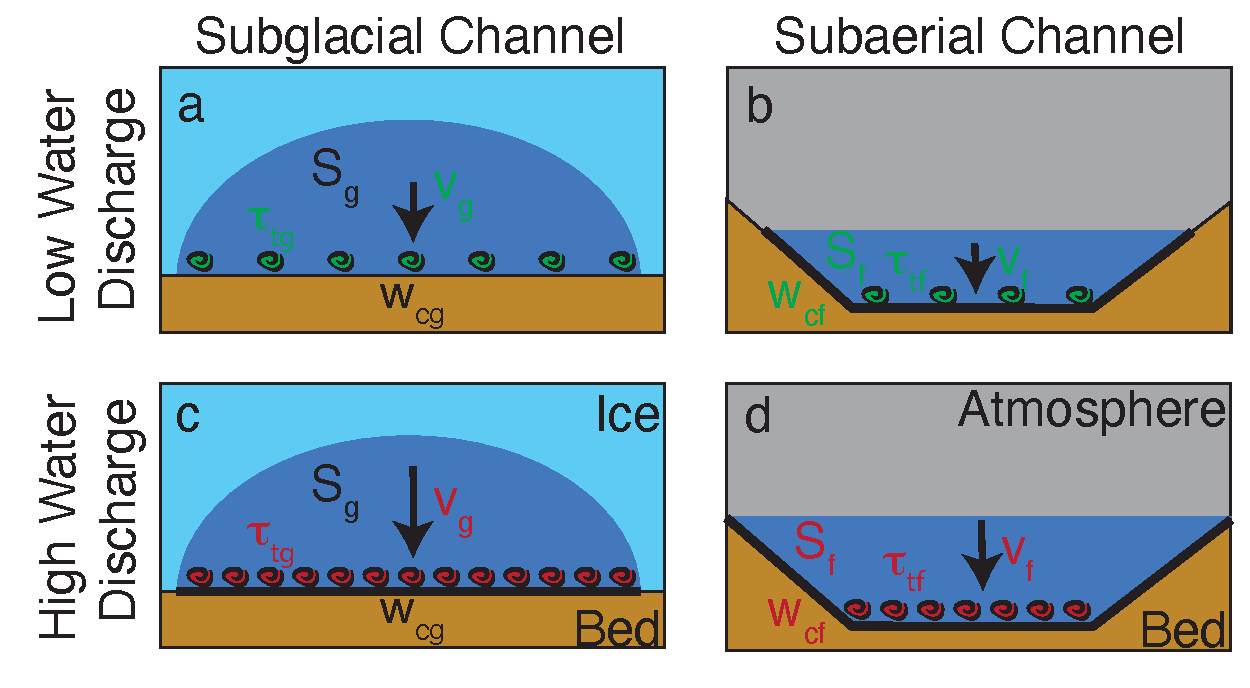
\includegraphics[width=0.8\linewidth]{Fig1.pdf}
    \caption{Sketch of the situation with various parameters. Water velocity magnitude in the subglacial, $v_g$, and subaerial, $v_f$, systems are shown by arrow length. $S_g$ and $S_f$ represent the cross-sectional area in subglacial and subaerial channels. The subglacial channel widths $w_{cg}$ remain steady, while the subaerial channel widths evolve $w_{cf}$, denoted by the thick black line. Shear stress $\tau$ is responsible for the mobilization of sediment and increases with the number of makers at the channel bed. 
      Note that in the subaerial channel parameterization, rectangular channel shapes are implemented (Section~\ref{sect:fluv}).} 
    \label{fig:cartoon}
  \end{figure}
\end{center}


\section{Methods}
\label{sect:meth}
Parameterizations below represent relationships amongst water discharge, subglacial water velocity, and channel geometry in both subaerial and subglacial channels (Table \ref{table:vpm}).
Because sediment transport largely depends on shear stress applied by water flow \cite{shields1936}, both parameterizations calculate this value and integrate  it across the channel bed (Figure \ref{fig:cartoon}).
The evaluation of shear stress omits a grain size parameter and, thus, leaves open the selection of a sediment transport relationship  \cite<e.g.>[]{shields1936,meyer1948} to  calculate sediment transport capacity.
As a result, relative relationships in shear stress, as opposed to sediment transport capacity, are examined.


\ian{update hooke angle }
\begin{table}[H]
  \centering
  \caption{Variables, parameters, and constants }
  \begin{tabular}{ l  c  c c }
    Name &Symbol&  Value&Units \\ \hline
    \textbf{Variables}  & & & \\
    Water discharge  & $Q_w$& & $\mathrm{m^{3}\,s^{-1}}$ \\
    Water velocity (glacier, subaerial)  & $v_g,\,v_{f}$& & $\mathrm{m\,s^{-1}}$ \\
    Channel cross-sectional area (glacier, subaerial) &  $S_g, S_f$& & $\mathrm{m^2}$     \\
    Hydraulic diameter &$D_h$&&$\mathrm{m}$\\
    Width of channel floor (glacial, subaerial) & $w_{cg},w_{cf}$&  & $\mathrm{m}$     \\
    Hydraulic head &$\Delta h$&& $\mathrm{m}$\\
    Shear stress (glacier, subaerial) & $\tau_g,\,\tau_f$&& $\mathrm{Pa \, m^{-1}}$ \\
    Width-integrated shear-stress (glacier, subaerial) & $\tau_{tg},\, \tau_{tf}$&& $\mathrm{Pa \, m^{-1}}$ \\

         &&&\\
    
    \textbf{Parameters and Constants}  & & &\\
    Gravitational constant&$g$& $-9.81$&$\mathrm{m\,s^{-2}}$\\
    Density of water & $\rho_w$& $1000$ & $\mathrm{kg\,m^{-3}}$ \\
    Density of ice & $\rho_i$& $900$ & $\mathrm{kg\,m^{-3}}$ \\
    Hooke angle of channel & $\beta$ & $\frac{\pi}{2}$ & \unit{rad}\\
    Effective glacier thickness &$h_o$& $225^a$ or $700^b$  &\unit{m}\\
    Effective glacier length &$l$&$7000^a$ or $20,000^b$&\unit{m}\\
    Constant $1$ &$C_1$&$2.2\times10^{-5}$&\unit{m}$^{-1}$\\
    Constant $2$ &$C_2$&$3.7\times10^{-13}$&\unit{m}$^{-n}\,s^{-1}$\\
    Latent heat of fusion &$L$&$333.5 $&\unit{kJ\,kg}$^{-1}$\\
    Pressure melting coefficient &$c_t$&$7.5\times 10^{-8}$&\unit{K\,Pa}$^{-1}$\\
    Specific heat capacity of water &$c_p$&$4180$&\unit{J\,kg}$^{-1}$\unit{K}$^{-1}$\\
    
    Ice flow constant &$A$& $5.3\times10^{-24}$ &\unit{Pa}$^{-n}$\,$s^{-1}$\\
    Ice flow exponent &$n$& $3$ &$\mathrm{(-)}$\\
    Friction factor (glacier) & $f_r$ & $4$ & $\mathrm{(-)}$ \\
    Friction factor (subaerial) & $f_p$ & $3$ & $\mathrm{(-)}$\\
    Gradient of channel bed (subaerial) &$\frac{\partial z_c}{\partial x}$ &$0.05$& $\mathrm{(-)}$\\
    Subaerial channel factor & $k$ &$3$ & $\mathrm{s\,m^{-2}}$\\
    Channel geometry exponent &$e$& $\frac{1}{2}$&$\mathrm{(-)}$ \\
    \hline
  \end{tabular}
  \label{table:vpm}

\end{table}
  $^a$ for Fieschergletscher
  
  $^b$ for Leverett glacier

\subsection{Subglacial channel  parameterization}
\label{sect:sub_mode}

To evaluate the shear stress of water flowing across sediments below a glacier, the subglacial channel parameterization evaluates the channel geometry and the velocity of the flowing water.
To accomplish this, a modified version of  the lumped hydraulics model presented in \citeA{clarke1996} and \citeA{werder2010} is used.

Here, it is assumed that the water is transported through a subglacial channel flowing down the glacier; \cite<Figure~\ref{fig:cartoon}; >{rothlisberger1972}, and that the channel  size responds to frictional heating from water flow and creep closure by ice, using the Darcy-Weisbach formulation for water-flow through a pipe  \cite<e.g.>[]{rothlisberger1972,clarke2003}.
In the formulation here does not consider englacial storage of water, and thus that changes in hydraulic head at the top of the glacier are negligable in the evolution of the channel size. 
The evolution of subglacial channel size $S_g$ is given as
\begin{linenomath*}
  \begin{equation}
    \label{eq:dS_dt}
    \frac{\partial S_g}{\partial t} = C_2 \frac{Q \Delta h}{l} - C_2 (h_{o}-\frac{\Delta h}{2})^n\,S_g,
  \end{equation}
\end{linenomath*}
\noindent $C_1= (1-\rho_wc_pc_t)\,\frac{\rho_wg}{\rho_iL}$ and $C_2=2A(\frac{\rho_wg}{n})^n$ are constants (Table \ref{table:vpm}), $l$ is the length of subglacial channel, $Q$ is water discharge, $\Delta h$ is the hydraulic potential change from the glacier terminus to its top, $h_{o}= \frac{\rho_i}{\rho_w} h_{ice}$ is the ice overburden pressure, and $n$ is Glen's n.
The first term on the right side of the equation represents the opening of the channel through frictional heating, while the second term represents the creep closure of the channel from ice deformation. 


Following the Darcy-Weisbach, head drop $\Delta h$ is,
\begin{linenomath*}
  \begin{equation}
    \label{eq:dh}
    \Delta h \,  = l \,\frac{1}{g}\,s\,f_r\,\frac{Q^2}{D_h^5}
  \end{equation}
\end{linenomath*}
\noindent where $f_r$ is a friction factor, $D_h$ is the hydraulic diameter, and $l$ is the length overwhich head change occurs. $s$ is a factor accounting for channel geometry \cite{hooke1990}, calculated as:
\begin{equation}
  \label{eq:Hf}
  s = \frac{2\,(\beta -\sin \beta)^2}{(\frac{\beta}{2}\,+\,\sin \frac{\beta}{2})^4},
\end{equation}
where $\beta$ is the central angle of the circular segment that comprises the channel (the so-called Hooke angle). Note that $\beta =\pi$ corresponds to a semi-circle and
smaller values of $\beta$ result in shallow, wide channels.

With knowledge of cross sectional area $S$, the shear stress, $\tau$, between the water and the channel bed is determined through the Darcy-Weisbach formulation
\begin{equation}
  \label{eq:tau}
  \tau_g=\frac{1}{8}\,f_r\,\rho_w\,v_g^2,
\end{equation}
% 
where  the water velocity $v_g = \frac{Q_w}{S_g}$.

The width of the flat channel floor $w_{cg}$, given angle $beta$ is 
\begin{equation}
  \label{eq:dh2wc}
  w_{cg} = 2  \sin \frac{\beta}{2} \sqrt{\frac{2\, S}{\beta -\sin \beta}}.
\end{equation}

Width integrated shear stress is represented as $\tau_{tg}=w_{cg}\,\tau_g $.

\subsection{Subaerial channel  parameterization}
\label{sect:fluv}

To parameterize the shear stress of water flowing across sediments in the subaerial channel,  the hydraulics parameterization presented in \citeA{tucker1997} is implemented.
Here, it is assumed that there is a conservation of mass and a sufficiently wide channel so that the hydraulic radius is consistent with flow depth, uniform flow, and the Darcy-Weisbach relationship.
The shear stress $\tau_f$ at the river bed is represented as
\begin{linenomath*}
  \begin{equation}
    \label{eq:DW_tau}
    \tau_f=\frac{\rho_w\,g^{\frac{2}{3}}\,f_p^{\frac{1}{3}}}{2}\, \Big(\frac{Q_w}{w_{cf}} \Big)^{\frac{2}{3}} \,\frac{\partial z_c}{\partial x}^{\frac{2}{3}},
  \end{equation}
\end{linenomath*}
where $\frac{\partial z_c}{\partial x}$ is the channel slope, and $f_p$ is the friction factor for subaerial systems.
Channel width $w_{cf}$ is 
\begin{equation}
  \label{eq:wcf}
  w_{cf} = k \, Q_w^e,
\end{equation}
% 
where $k$ is a constant and $e$ is an exponent commonly equal to $\frac{1}{2}$ \cite{leopold1953}.
Water velocity, $v_f$, is given by rearranging Equation \ref{eq:tau} as
\begin{equation}
  \label{eq:vf}
  v_f = \sqrt{\frac{8\,\tau_f}{f_p\,\rho_w}}.
\end{equation}
% 
As in Section~\ref{sect:sub_mode}, the width integrated shear stress is $\tau_{tf}=w_{cf}\,\tau_f$.

\subsection{Implementation}

The parameterizations above are applied to hydrological records from the Fieschergletscher in the Swiss Alps (info) and the Leverett glacier on the Greenland Ice Sheet (info).
The hydrographs applied to the subglacial and subaerial parameterizations represent the subglacial flow of water as it leaves the glacier and moves into a subaerial flow in front of the glacier, as water moves through the catchment.
Outputs of the parameterizations are meant to represent generalizable sediment transport characteristics from these hydrographs, rather than actual hydraulic conditions.

The formulation of the glacial system (Section~\ref{sect:sub_mode}) requires inputs of the ice thickness ($h_o$, Equation\,\ref{eq:dS_dt}), water discharge, $Q_w$,  Hooke angle (Equation~\ref{eq:Hf}; $\beta$), and friction factor (Equations~\ref{eq:dh}~and~\ref{eq:tau}; $f_r$). Values of these parameters are given in Table~\ref{table:vpm}.

In the subaerial system,  only the bed slope, $\frac{\partial z_c}{\partial x}$, is needed in Equation~\ref{eq:DW_tau}. The friction factor, $f_f$, and channel shape factor, $k$, are assigned such that they produce reasonable values for water velocity and channel width  (Section~\ref{sect:fluv}).

The parameterizations are first applied to a reference test case for each glacier that assumes a semi-circular subglacial channel ($\beta=\pi$) and friction factors $f_r$ and $f_p$ are tuned so that the model reproduces reasonable velocities for both  the Greenland Ice Sheet and alpine glaciers \cite<$\sim\,1.6\,$\unit{m}$^3$\,\unit{s}$^{-1}$>{werder2010b,chandler2013}.
Water velocity, shear-stress and width-integrated shear-stress in the subglacial and subaerial systems are presented below.

To characterize the variability in sediment discharge capacity in subglacial compared to subaerial systems further, the parameterizations are applied to range of different channel geometry factors ($\beta$ and $k$) and friction factors $f_r$ and $f_p$.
Model runs with parameter combinations  are culled, if their maximum subglacial water velocity exceeds $2\,$\unit{m}$^3$\,\unit{s}$^{-1}$ or if subaerial water velocity exceeds $1\,$\unit{m}$^3$\,\unit{s}$^{-1}$.
The standard deviation of water velocity, shear-stress and width-integrated shear-stress across the season long hydrographs are presented below.


\section{Results}

% there is more variability across the season subglacial and subaerial cases. peaks in subaerial cases lag peaks in subglacial cases. (Figure 2)

% For a fixed channel geometry, there is a single shear stress for a water discharge. In the subglacial case, peak water discharge that is 1.5 times the mean velocity. In Fieschercase, peak water discharge does not result in the greatest of any variable. In Leverett case the mean total shear stress can occur from 100 m3/s to 200 m3/s. The mean velocity and shear stress can occur across effectively all water discharges below 250 m3/s

% across a wide range of channel geometries 

 
Following the parameterizations defined in Sections~\ref{sect:sub_mode}~and~\ref{sect:fluv}, the water velocity, shear-stress and total shear-stress exhibit vastly different seasonal evolutions and peaks of water velocity and shear stress (representing the potential for sediment mobilization) and total shear stress (representing the total sediment transport capacity; Figure~\ref{fig:model_outs}).
Furthermore, these variables respond differently to water discharge in the subglacial and subaerial systems (Figure~\ref{fig:Qw_vari}).
For each water discharge value in the subaerial system, there is a single water velocity, shear-stress and total shear-stress (Figure~\ref{fig:Qw_vari}).
In the subglacial system, water velocity, shear-stress and total shear-stress vary substantially for a given water discharge(Figure~\ref{fig:Qw_vari}).
For instance, over $15$ minute time periods at Fieschergletscher, the range of water velocities and shear-stress spans from those below the mean to those over $1.5$ times the mean.
Substantially high values of water velocity and shear-stress can occur from minimal water discharge at $2.5$\,\unit{m}$^3$\,\unit{s}$^{-1}$ to the maximum water discharge at over $17$ \,\unit{m}$^3$\,\unit{s}$^{-1}$.
At Leverett glacier, reduced diurnal variability in the hydrograph  (Figure~\ref{fig:model_outs} e) results in smaller variations in water velocity and shear stress compared to Fieschergletscher (Figure~\ref{fig:Qw_vari}).
However, mean values of water velocity can occur at water discharges between roughly $50$ \,\unit{m}$^3$\,\unit{s}$^{-1}$ and $225$ \,\unit{m}$^3$\,\unit{s}$^{-1}$, effectively spanning the observed water discharge. 

When accounting for the evolving channel width of the subglacial conduit, total shear-stress generally increases with water discharge.
Yet the total shear-stress across the can very substantially, with the highest values in total shear-stress occurring at water discharge values ranging from roughly $11$ \,\unit{m}$^3$\,\unit{s}$^{-1}$, to the maximum water discharge at over $17$ \,\unit{m}$^3$\,\unit{s}$^{-1}$.
The variance is less at the Leverett glacier case, yet a range of total shear-stress can occur at a given discharge(Figure~\ref{fig:Qw_vari} c, e).

Over the course of the season, large peaks in water velocity and shear stress, along with total shear stress, occur in response to increases in water discharge.
In the subglacial system, these peaks generally occur over the period when water discharge increases at the fastest rate (Figure~\ref{fig:model_outs}).
Conversely, in the subaerial system peaks in these variables occur when water discharge is at its highest value.
As a result, peaks in the subglacial variables occur prior to the peaks in the subglacial variables, representing lags sediment mobilization and  transport capacity as sediment is transferred from on system to the other.

The water velocity and shear stress remain higher across the different friction factors and channel geometries examined in the ensemble of runs across averaging periods.
However, the Leverett case, some parameter combinations the result in greater variability in subaerial system compared to the subaerial channels.
The effect of channel evolving width largely counteracts the variability in water velocity, especially in the alpine glacier case.
Here the large diurnal cycles in the hydrograph can cause the maximum and minimum amounts of variability in subaerial total shear-stress to be greater than those in the subglacial system.
At the Leverett glacier, with reduced diurnal variability in water discharge (Figure\,\ref{fig:model_outs}), the variability in total shear-stress remains higher in the subglacial system compared to the subaerial one.
However, some variability in subaerial parameter combinations exceeds those subglacial ones.
Note however, that this occurs across the total of xxx parameter combinations examined.









\begin{center}
  \begin{figure}[H]
    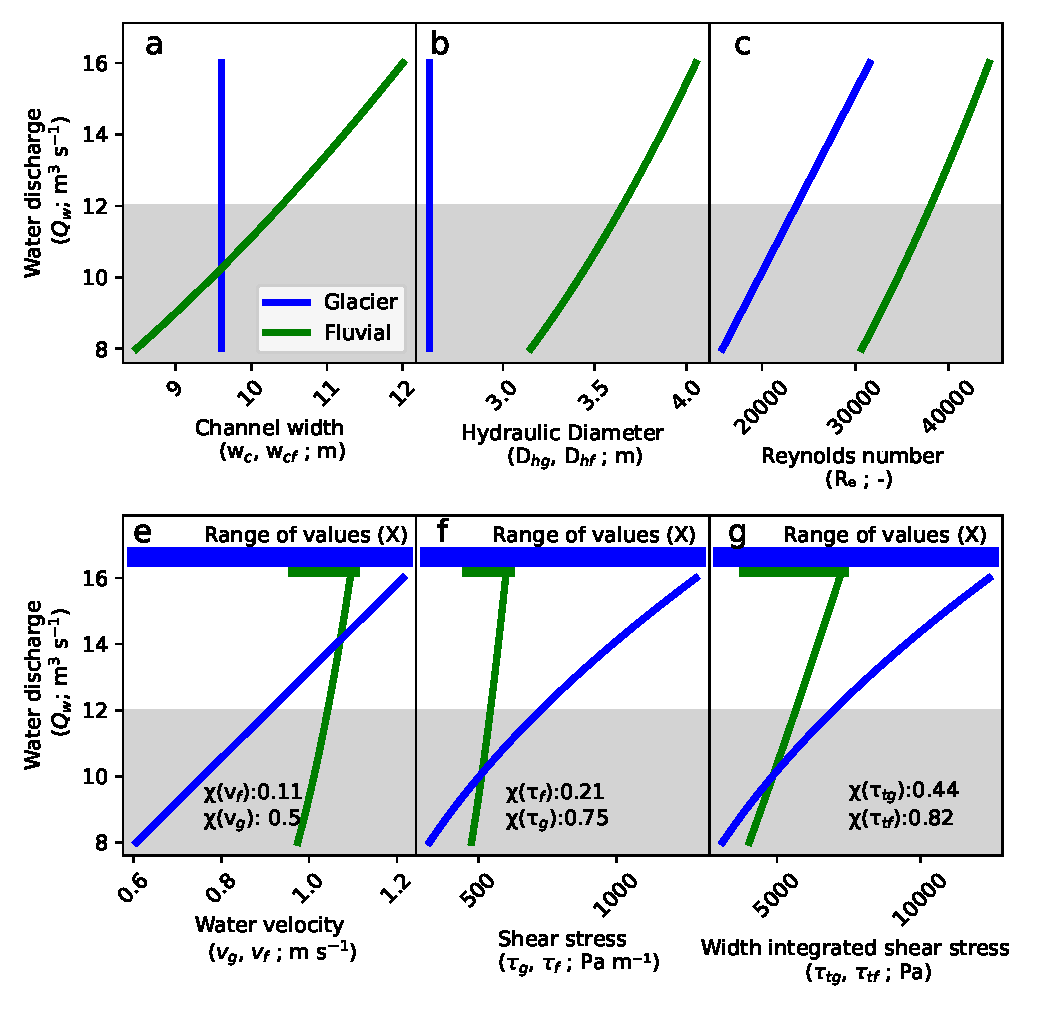
\includegraphics[width=0.8\linewidth]{model_outputs.pdf}
    \caption{Model outputs as in response to hydrograph (a and e) from Fieschergletscher (a-d) and Leverett glacier (e-h). Gray line in a and e represent subglacial channel cross sectional area. Below this black lines represent model outputs of velocity, shear-stress and width-integrated shear-stress from the subglacial system, while grey lines represent the subaerial system. } 
    \label{fig:model_outs}
  \end{figure}
\end{center}


\begin{center}
  \begin{figure}[H]
    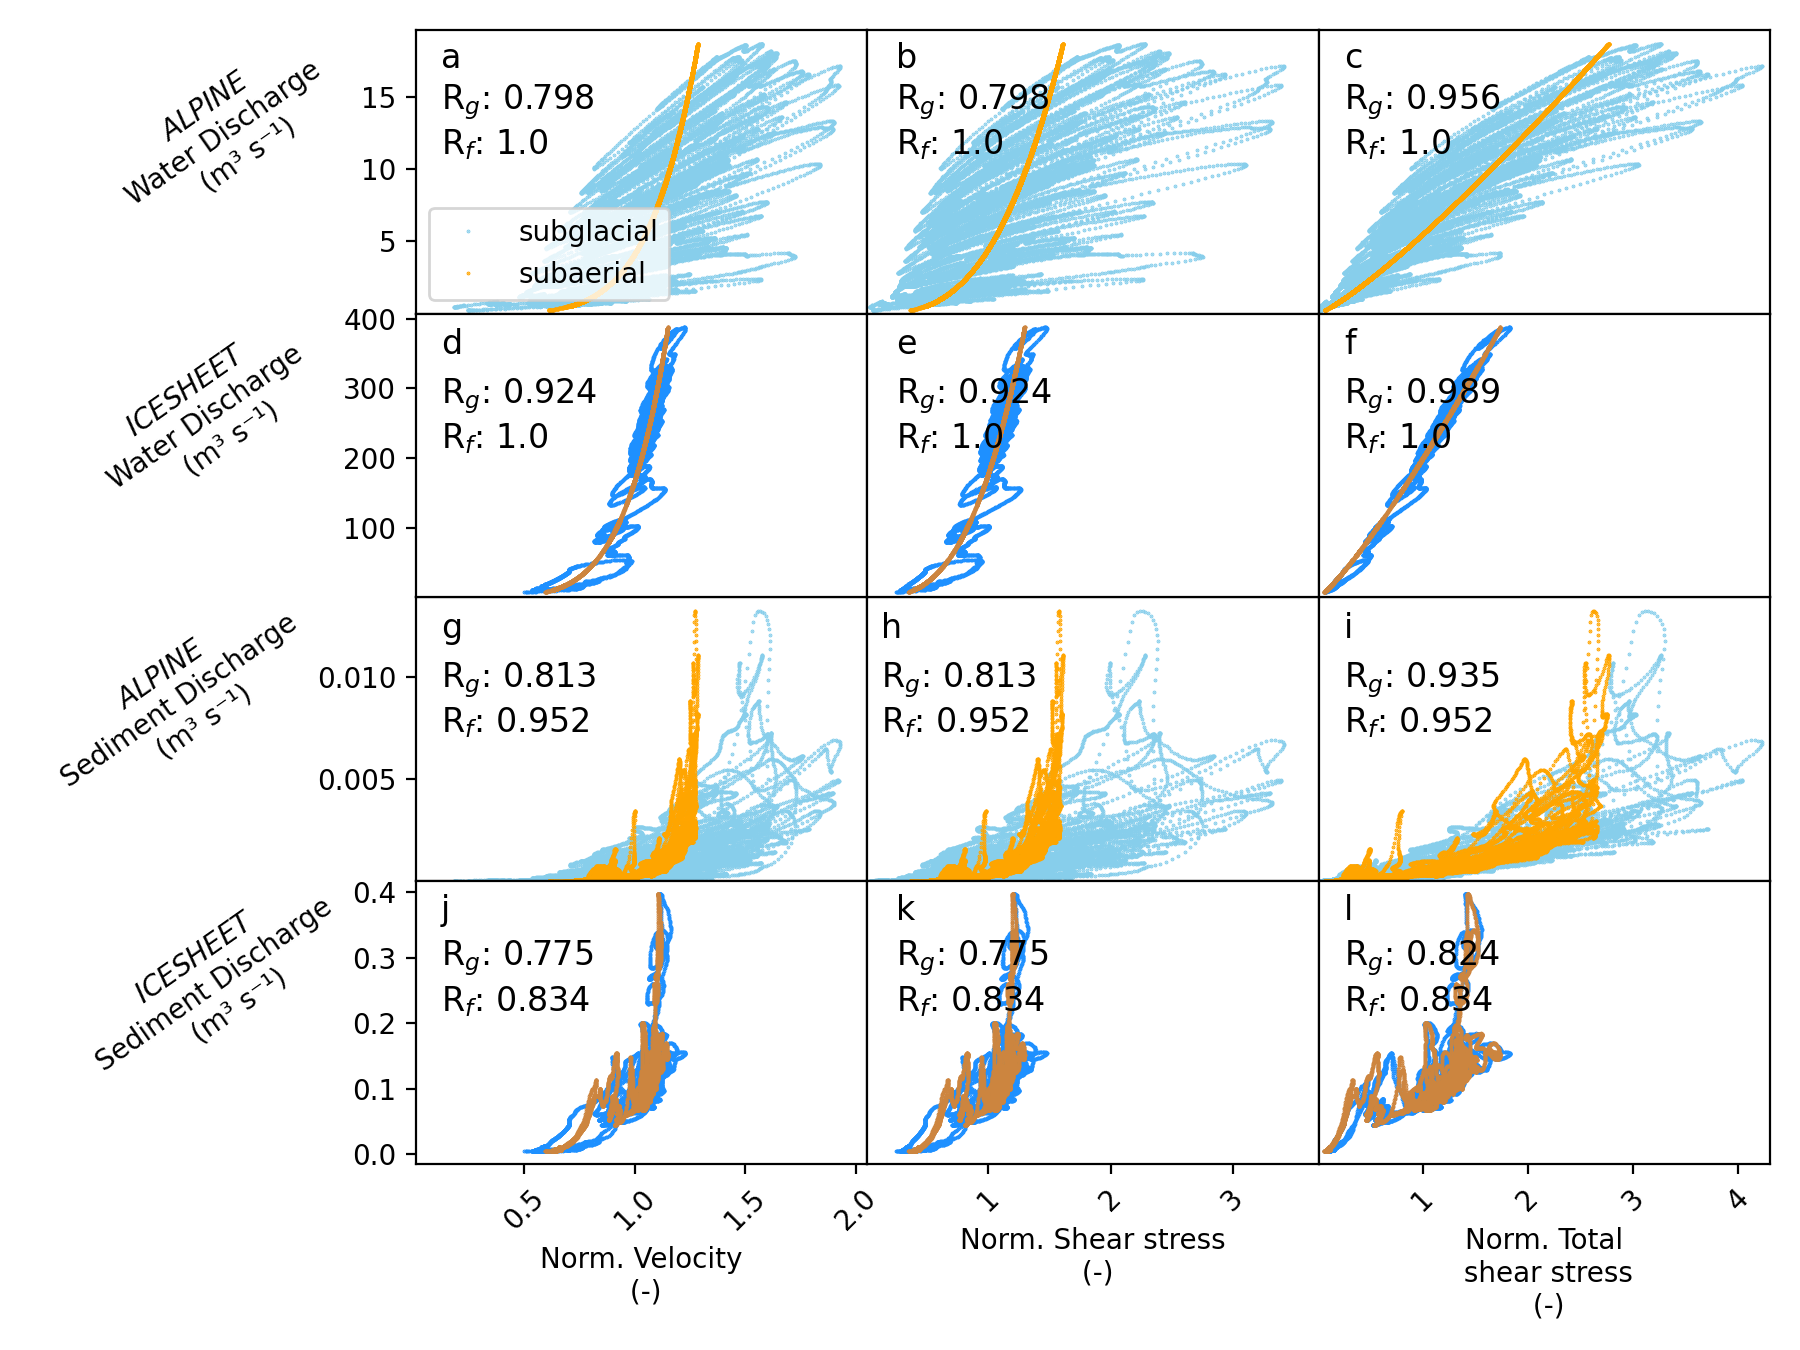
\includegraphics[width=0.8\linewidth]{Qw_vari.png}
    \caption{Relationship between water discharge and velocity, shear stress and width-integrated shear stress for the Fieschergletscher hydrograph (a-c) and Leverett glacier (d-f). Variables have been normalized to by the mean values for better comparison amongst the model runs.} 
    \label{fig:Qw_vari}
  \end{figure}
\end{center}


\begin{center}
  \begin{figure}[H]
    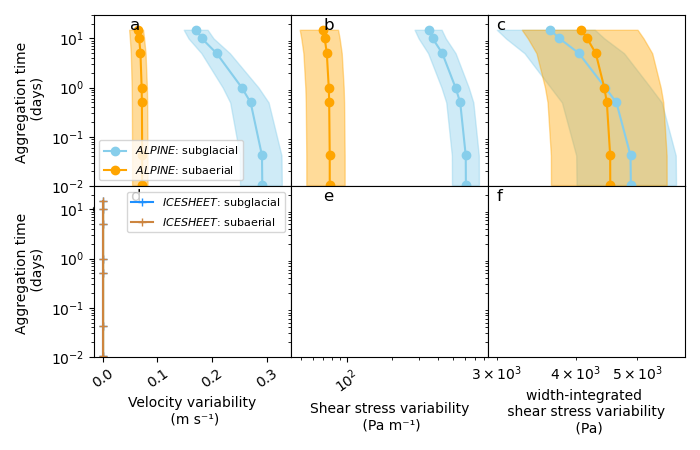
\includegraphics[width=0.8\linewidth]{multi_run.png}
    \caption{} 
    \label{fig:multi_run}
  \end{figure}
\end{center}

\section{Discussion}
\ian{add cautionary note as this is an example}

\ian{Zwally and tedstone effect with increased discharge... non-linear response of increasing water discharge. }

The relationship between water discharge variability and relative variability of the water velocity, shear stress, and width-integrated shear stress results from the fixed geometry in the glacier system and variable geometry in the subaerial system as they respond to changes in water discharge (Equations~\ref{eq:tau_t} and \ref{eq:v}).
Increased variability in sediment transport capacity with respect to discharge has several implications for sediment transport in subglacial systems compared to subaerial ones.
Shear stress is scaled to the $\frac{3}{2}$ power and relies on shear stress exceeding a threshold in sediment transport relationships  such as in \citeA{meyer1948}.
In the total sediment transport relationship \citeA{engelund1967}, the shear stress is scaled to $\frac{5}{2}$ power.
In both cases, the exponent greater than $1$ of shear stress in the sediment transport relationship magnifies the variability in sediment transport beyond the highly variable shear stress and width-integrated shear stress described above in subglacial environments (Figure~\ian{xxx}).

% Both subglacial and subaerial parameterizations here assume that the distribution of velocity and shear stress of water across the channel bed is homogeneous \cite<Section~\ref{sect:sub_mode}~and~\ref{sect:fluv}; e.g. >{yager2018}.
% \ian{Phillips and Jeromack 2016... stabilization here.}
% In the subaerial parameterization, this means that sediment is transported across all channel widths, as opposed to large flows such as floods when much sediment transport occurs \cite{wolman1960}.
% As a result, the  the subaerial systems variability in sediment transport capacity across the range of discharge values could be underestimated in the parameterization here (Figure~~\ian{xxx}).

\subsection{Sediment transport below glaciers and at their margins}

The response of sediment discharge caused by the greater variability in sediment transport in subglacial channels will be greatest in completely transport-limited regimes \cite<e.g.>[]{kasmalkar2019}.
In supply-limited systems, the changing sediment transport capacity (Figure~\ref{fig:model_outs}) would have a minimal effect on sediment discharge due to the absence of sediment available for transport \cite{delaney2019}.
Yet, in the subglacial system reaching the threshold of motion for sediment frequently, across a range of discharges,  may result in additional sediment transport.
The variable sediment transport capacity may result in a tendency for glaciers to evacuate sediment and transition to a supply-limited regime whereby sediment discharge scales with glacier sliding  \cite<e.g.>[]{herman2015}.
Sediment exhaustion by this process may also explain the dependence of sediment discharge from the Greenland Ice Sheet on basal shear stress, a proxy for bedrock erosion, as opposed to glacier melt \cite{overeem2017}.

The effect of pressurized channel flow could be most pronounced during precipitation or flood events when subglacial conduits have not adapted to the water discharge flowing through them, resulting in a large increase in sediment transport capacity and discharge \cite<e.g.>[]{cowan1988,delaney2019}.
Exceptional sediment discharge during floods may result from changes to sediment access below the glacier, yet rapid increases in water velocity from water flowing through a small channel will also cause a large increase in sediment transport capacity, not possible in a subaerial system (Section~\ref{sect:sub_mode}).

Increased variability in sediment transport may also impact sediment export from the subglacial environment into proglacial areas \cite<e.g.>[]{perolo2018}.
Here, velocities at the highest water discharges could generally decrease (Figure~\ref{fig:model_outs}, blue and green horizontal bars), in the transition of pressurized subglacial flow to subaerial open-channel flow as the water leaves the glacier. The decrease in water velocity potentially results in sediment deposition once sediment enters the proglacial area.
Periodic sediment deposition in sediment deposition may even result in the transition between pressurized and subaerial flow below the glacier terminus \cite{perolo2018}, especially when cavity closure rates of the ice are slow \cite{egli2021b}.

In large catchments and further downstream of proglacial margins, water discharge is generally less variable than at the tops of catchments, where glaciers lie in
alpine settings \cite<c.f.>{swift2005,riihimaki2005,costa2017,vanas2017}.
Here, external hydrological factors further downstream of glaciers could result in smaller variations in sediment transport capacity in many subaerial systems compared to subglacial ones.

The parameterization here shows that the smallest variability in water discharge has the largest difference in relative variability in sediment transport metrics (Figure~~\ian{xxx}).
At locations such as the Greenland Ice Sheet, smaller diurnal variations in water discharge compared to many alpine catchments \cite<c.f.>{swift2005,riihimaki2005,vanas2017,hasholt2018}.
Therefore, the variability in sediment transport capacity in the transition from the ice sheet to the proglacial river could be more dramatic in Greenland than in alpine systems as water leaves the glacier and moves downstream.
Thus the disparity in sediment transport capacity between the subglacial and subaerial systems could be most pronounced in larger catchments, potentially resulting in temporally mismatched periods between when glaciers introduce sediment to these river systems  and when the river mobilizes it (Figures~\ref{fig:model_outs}).


\subsection{Records of sediment discharge  from glaciers}

\ian{include comments about the limits of hysterisis analysis from glacial systems}

Large variations in sediment transport capacity below glaciers may result in sediment mobilization and deposition processes in close spatial and temporal proximity to each other below the glacier \cite{gimbert2016,perolo2018}.
The rapid increase and decreases in sediment transport capacity, for example over a diurnal cycle, in a subglacial system may compound the variability in sediment transport already present in subaerial systems \cite{williams1989,jerolmack2010}.
As a result, variations in sediment transport capacity could be responsible for the fluctuations in sediment discharge (``flushings'') from glaciers that are not attributed to variations in water discharge \cite<e.g.>[]{richards2003,swift2021}.
Aside from the sporadic nature of these events, the observed ``flushings'' could result from increases in water velocity resulting from reduced channel size, not water discharge, which increase sediment transport capacity.

Additional processes and erosional hiatuses may further complicate signals of sediment discharge from glaciers in response to climate, compared to subaerial systems \cite{jansson2005,ganti2016}. 
For instance, sediment transport capacity from a glacier reacts to the ice thickness, controlling the closure of the channel, and the surface slope of the glacier, controlling water velocity \cite<Section~\ref{sect:sub_mode}; >{rothlisberger1972,shreve1972,delaney2022,stevens2022}, in addition to water discharge.
Conversely, sediment transport in most subaerial systems increases with water discharge and hydraulic gradient, and the hydraulic gradient probably remains relatively stable over yearly to century-scale time periods \cite<Section~\ref{sect:fluv}; e.g.>{muller1968,whipple1999,wong2006,wickert2019}. 

Records of sediment discharge have been used to establish the relationship, or lack thereof, between sediment discharge and climate in glacial systems \cite<e.g.>[]{koppes2009a,willenbring2016,mariotti2021}.
The variability in subglacial sediment transport capacity presented here applies most generally to short-time scales responsible for the size of subglacial channels.
Yet, identifying climatic signals in sediment transport from transport-limited glaciers may require higher thresholds of climatic perturbation compared to subaerial systems \cite{tofelde2021}.
This higher threshold of climatic perturbation may persist in addition to the stochastic nature of erosion and deposition in fluvial environments \cite{castletort2003,jerolmack2010,romans2016}.
For instance, sediment discharge records from two glaciers in the Swiss Alps show that $40$ to $50$\% of a season's sediment discharge occurs when water discharge is below the $75^{\mathrm{th}}$ quantile of the season \cite{delaney2018}.
Such a large quantity of sediment transported at lower water discharges may occur in part because sediment transport capacity responds to the size of the glacier conduit, in addition to water discharge (Section~\ref{sect:sub_mode}).

This suggests that a larger climatic perturbations in water discharge might be needed to isolate significant changes sediment discharge from glacial systems compared to subaerial on, as the noise resulting from increased variability in sediment transport capacity must be overcome.
Furthermore, if no sediment is available and the glacier is in a supply-limited case, then the sediment discharge record will also represent additional processes of bedrock erosion from  water pressure variations and sliding  \cite{iverson2012,herman2015}, which are also complex.


\section{Conclusions}
Subaerial channels can alter their channel width and water velocity in response to changing water discharge.
Conversely, pressurized subglacial channels accommodate changing water discharge by altering water velocity and shear stress, upon which sediment transport depends.
This occurs because the size of subglacial channels evolves slowly compared to variations in water discharge.

Parameterizations of subglacial and subaerial water flow show that subglacial systems exhibit increased variability in sediment transport capacity as they respond  to changes in water discharge.
The variability in sediment transport capacity is reduced when the evolving channel width is accounted for in subaerial systems.
Even so, variability in sediment transport capacity across a channel's width is consistently higher in subglacial channels compared to subaerial ones.


The differences in subglacial and subaerial channels' response to variations in water discharge should be considered when examining sediment transport processes in glacierized catchments.


\section*{Open Research}
\noindent
The julia code used herein is included in the supplementary material.



\acknowledgments
I was funded by SNSF Project No. PZ00P2\_202024.


%% ------------------------------------------------------------------------ %%
%% References and Citations

%%%%%%%%%%%%%%%%%%%%%%%%%%%%%%%%%%%%%%%%%%%%%%% 
% 
% \bibliography{<name of your .bib file>} don't specify the file extension
% 
% don't specify bibliographystyleiz

% In the References section, cite the data/software described in the Availability Statement (this includes primary and processed data used for your research). For details on data/software citation as well as examples, see the Data & Software Citation section of the Data & Software for Authors guidance
% https://www.agu.org/Publish-with-AGU/Publish/Author-Resources/Data-and-Software-for-Authors#citation

%%%%%%%%%%%%%%%%%%%%%%%%%%%%%%%%%%%%%%%%%%%%%%% 

\bibliography{Paperlib.bib}


% \section{Supplement}

% \renewcommand{\figurename}{Figure S}
% \setcounter{figure}{0}

% \begin{center}
%   \begin{figure}[H]
%     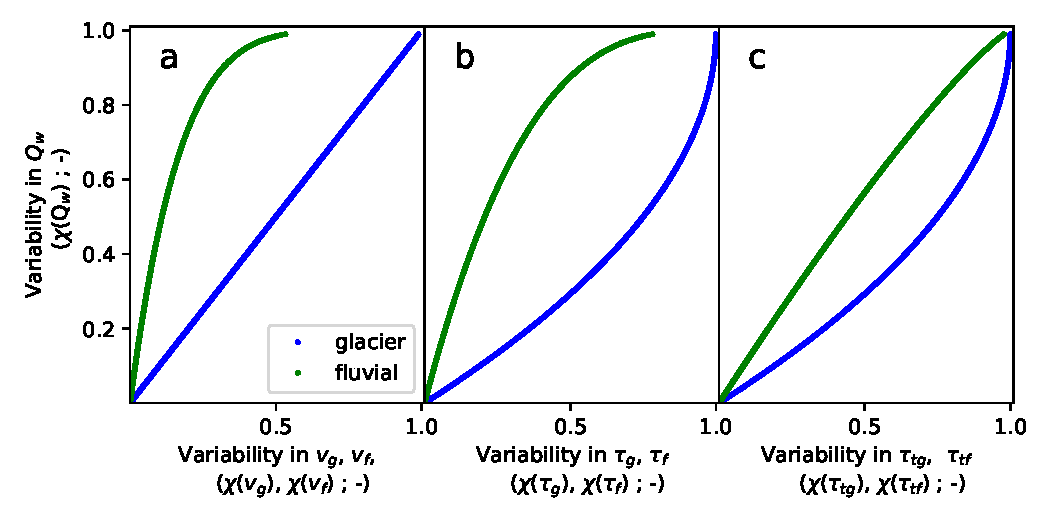
\includegraphics[width=0.8\linewidth]{multi_run_vars.pdf}
%     \caption{Variability $\chi$ in velocity ($v_g$, $v_f$; a) shear stress ($\tau_g$, $\tau_f$; b) and width-integrated shear stress ($\tau_{tg}$, $\tau_{tf}$; c)  in glacial and subaerial systems. Values are determined from examining the same parameter space in Figure~\ref{fig:range}. }
%     \label{fig:gammas}
%   \end{figure}
% \end{center}


\end{document}

These different characteristics between glacial and subaerial channels show that records of sediment transport downstream of glaciers represent both subglacial and subaerial processes together.
Divergent processes discussed here might be particularly relevant at glacier margins, where water transitions from pressurized subglacial flow to open-channel subaerial flow.
The inconsistent response of sediment transport in subglacial and subaerial systems to changing water discharge could add uncertainty in evaluating  sediment transport signals in subglacial systems.
In addition, the subglacial parameterization shows that sediment transport capacity in glacier systems responds to a large number of factors such as channel size, ice thickness, and glacier surface slope, which may react to climate forcing differently than water discharge alone.
